\RequirePackage[T1]{fontenc}
\documentclass[conference]{IEEEtran}
\usepackage{cite}
\usepackage{amsmath}
\usepackage{graphicx}
\usepackage{booktabs}
\usepackage{array}
\usepackage[hidelinks,pdfversion=1.7]{hyperref}
\hypersetup{pdftitle={Persona-Aware, Knowledge-Bounded NPC Dialogue Through Model-Agnostic LLM Orchestration},pdfauthor={Mohan Chandra S S, Shreyas C, Nithish Gowda H N, Nithin S}}
\begin{document}
\title{Persona-Aware, Knowledge-Bounded NPC Dialogue Through Model-Agnostic LLM Orchestration}
\author{\IEEEauthorblockN{Mohan Chandra S S, Shreyas C, Nithish Gowda H N, Nithin S}
\IEEEauthorblockA{RV University\\USNs (in author order): 1RVU23CSE282, 1RVU23CSE443, 1RVU23CSE317, 1RVU23CSE316}}
\maketitle
\begin{abstract}
NPC dialogue requires coordinated persona, world knowledge, conversation context and response delivery rather than unrestricted text generation. We present Anima, an implemented orchestration architecture that combines deterministic engagement, persona-aware appraisal, source-bound retrieval, acknowledged dialogue history, a common model-provider contract and bounded response acceptance. A new evaluation uses 24 interconnected fictional world documents, indexed as 24 source chunks and separately as a 21-chunk authorized reference anthology. Six four-turn conversations produced 24 accepted real-model replies across three existing personas. Sequential traces preserve one, two and three prior exchanges in follow-up prompts. An assistant-coded qualitative audit examines support and referents without claiming independent human ratings; it also identifies unsupported elaboration and a secrecy presupposition. On 24 predeclared source-lookup queries, designated-source Precision@1 was 0.833, Recall@3 was 1.00 and mean reciprocal rank was 0.917. Thirty warm retrievals averaged 18.15 ms. Index synchronization exposed an edited fact without a generator-training step. Native Skyrim records demonstrate authored delivery and generated-response staging, while visible generated gameplay and audible playback remain unverified. The results support reusable orchestration mechanisms, not universal model equivalence or guaranteed semantic containment.
\end{abstract}
\begin{IEEEkeywords}
non-player characters, persona conditioning, retrieval-augmented generation, model abstraction, knowledge boundaries, dialogue evaluation
\end{IEEEkeywords}

\section{Introduction}
Non-player character (NPC) dialogue must respond to a player's request without abandoning the character's identity, obligations, or knowledge. Authored dialogue gives predictable control, but broader coverage requires additional content and branching logic. Language models supply flexible realization; fluency alone, however, does not establish that an NPC knows a fact or should engage. Game-dialogue research already motivates conditioning on character, history, and state~\cite{callison2022}.

Game knowledge changes independently of model behavior: locations and character facts may be revised while an inference backend remains fixed. Character training~\cite{shao2023} and parameter-efficient adaptation~\cite{hu2022} remain legitimate strategies. External retrieval~\cite{lewis2020} offers a complementary maintenance mechanism by supplying updated domain facts during inference rather than requiring an application training operation.

Anima places a dedicated orchestration layer between interaction interfaces and model inference. The layer appraises persona and trusted state, chooses authored/end/generated routes, retrieves source-bound evidence when needed, and validates model output under deadlines. Its contribution is the integration of these boundaries, not the invention of RAG, persona prompting, or provider abstraction. The term knowledge-bounded describes the architecture's intended access and acceptance controls; it does not assert guaranteed semantic faithfulness.

Our contributions are the implemented policy-controlled composition, traceable multi-turn knowledge conversations, explicit provider and source boundaries, and native Skyrim delivery evidence. The experiments examine coordinated behavior without claiming new retrieval or memory algorithms. Small authored datasets, one real model and non-independent semantic assessment constrain generalization.

\section{Related Work}
RAG combines parametric generation with nonparametric retrieved memory~\cite{lewis2020}. Anima supplies passages to an external inference model rather than training the RAG components. Dense passage retrieval establishes representation-based candidate selection~\cite{karpukhin2020}; our implementation uses an existing MiniLM encoder and cosine search, not a new retrieval objective.

Character-LLM adapts characters through profiles and experiences~\cite{shao2023}. Anima instead keeps authored personas and current state outside generator parameters. This does not establish superior character quality or training-cost savings; LoRA~\cite{hu2022} is a relevant efficient adaptation alternative.

Generative Agents already orchestrates memory, retrieval, reflection, and planning~\cite{park2023}. Consequently, the defensible contribution here is a particular policy-controlled integration with explicit trust, evidence, and timing boundaries, rather than a first unified agent framework. Game-state-aware dialogue is also established~\cite{callison2022}. Anima focuses on reusable runtime composition, without reproducing autonomous town simulation or a trained gameplay model.

Profile-conditioned dialogue is established by Persona-Chat~\cite{zhang2018}; an authored profile alone is neither a new method nor evidence of sustained persona consistency. Anima adds runtime source authorization, deterministic route selection and game delivery around that conditioning.

Evaluation must separate retrieval relevance, faithful evidence use, and generation quality, as emphasized by RAGAs~\cite{es2024}. Long-context availability does not guarantee reliable context utilization~\cite{liu2024}. Our literal answer-target diagnostic therefore cannot substitute for independent claim-level support or persona evaluation.

\section{Problem Formulation and Research Contributions}
For utterance $u$, trusted snapshot $s$, observations $o$, persona $p$, acknowledged history $H$, and external documents $D$, appraisal constructs $c=A(u,s,o,p,H)$ and policy selects $a=\pi(c)$. A generated route retrieves $E=R(q(c),D,b)$ under trusted source binding $b$, constructs prompt $P=B(c,a,E)$, and obtains candidate $y=G_\theta(P)$. Acceptance $V(y,c,a,E)$ controls whether the response leaves the runner. Here $q$ resolves the retrieval question, $b$ is the authorized source binding, $B$ packs the prompt, and $G_\theta$ is the selected generator. Authored/end routes bypass retrieval and inference.

We ask: \textbf{RQ1}, how does the implemented pipeline coordinate knowledge and acknowledged context across connected turns? \textbf{RQ2}, how well does retrieval rank predeclared sources, and what support limitations remain in generated replies? \textbf{RQ3}, how do authored personas and unknown-information boundaries appear in the resulting conversations? \textbf{RQ4}, where does the common contract separate orchestration from provider-specific inference? \textbf{RQ5}, can external knowledge be revised and accepted output reach a native game receiver? RQ1--RQ3 use exploratory traces and retrieval measurements, not a validated human-quality score. RQ4 is an architectural assessment; RQ5 separates retrieval updating from native lifecycle evidence.

The implementation contribution comprises deterministic engagement before model work, separation of trusted observations and untrusted references, source-bound retrieval with prompt-level evidence accounting, bounded candidate acceptance through a provider-neutral interface, and revision-correlated native game delivery. Model agnosticism is restricted to that interface and compatible transports. Incompatible APIs require an adapter, and model capabilities remain consequential.

\section{Proposed System Architecture}
Fig.~\ref{fig:architecture} presents the implemented component boundaries. The central \texttt{PreviewRunner} composes policy, context, optional retrieval, provider invocation, validation, and one permitted repair. The local lab and Skyrim connector invoke the same core rather than separate dialogue engines.

\begin{figure*}[t]
\centering
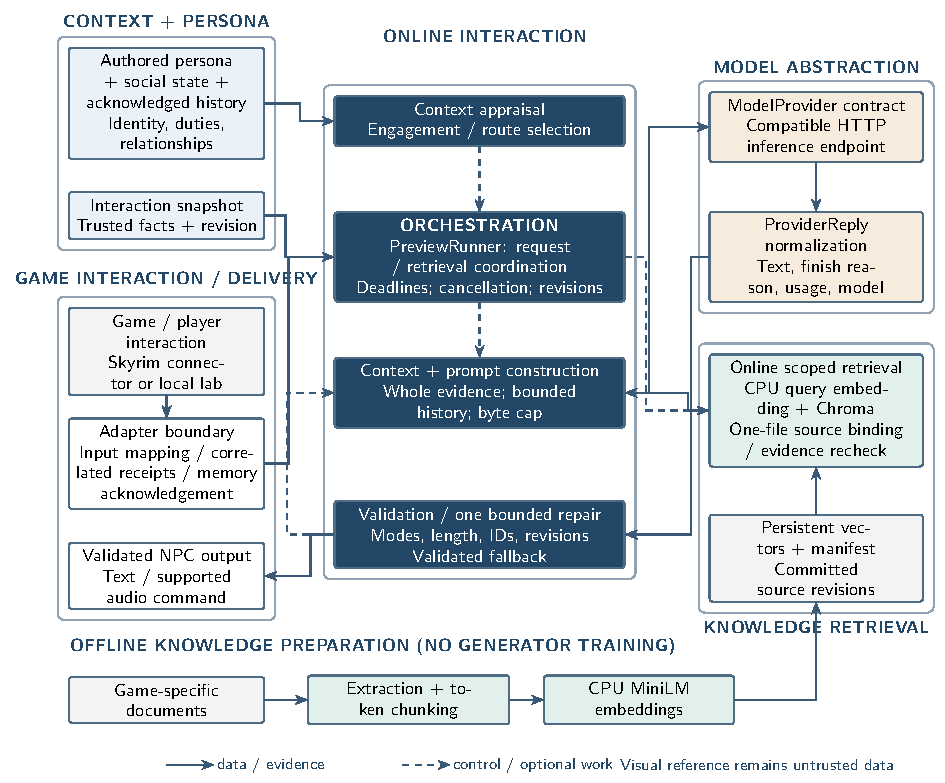
\includegraphics[width=.88\textwidth]{figures/system_architecture.pdf}
\caption{Policy-controlled architecture linking game interaction, knowledge access and response acceptance. Grouped boundaries separate interaction, persona/context, central orchestration, retrieval and provider normalization. Solid arrows carry data/evidence; dashed arrows denote control or optional work. Offline preparation is separate from inference. Native delivery is evaluated separately from retrieval and inference quality.}
\label{fig:architecture}
\end{figure*}

Appraisal verifies scope/revision and filters observations by perceiver, subject, confidence, and freshness. Conflicting equal-rank observations remain unknown. Persona and relationships influence tone and willingness, while familiarity does not grant knowledge. Deterministic policy can select authored greetings/refusals or end interaction before calling a model.

Retrieval is restricted by configured game/world/NPC file bindings; approximate similarity does not itself authorize a source. Prompt packing rechecks evidence and preserves whole passages. The provider contract contains messages, text, model identity, finish reason, and usage rather than vendor-specific orchestration policy. Candidate output cannot directly mutate quests, inventory, or relationships.

SocialStore persists revision-checked relationships and up to eight acknowledged exchanges. The lab commits display acknowledgements; current Skyrim composition can commit correlated completed native receipts with game-completed provenance. Interrupted or failed turns are excluded from completed history. Neither acknowledgement proves hearing. A durable production outbox and complete save-history reconstruction remain outside this slice.

\section{System Methodology}
\subsection{Offline Knowledge and Online Retrieval}
Loaders extract text from supported plain-text, structured, PDF, DOCX, and HTML files; OCR is not implemented. Encoder token offsets form default 220-token chunks with 32-token overlap. The all-MiniLM-L6-v2 sentence encoder~\cite{minilm2020,minilm_model} runs through ONNX Runtime~\cite{onnxruntime} and produces 384-dimensional CPU vectors. Chroma~\cite{chroma} stores cosine-search vectors with source/revision metadata. File hashes include content and pipeline parameters; a manifest publishes a replacement only after that file's batches succeed. Index synchronization is explicit, outside dialogue turns.

Online retrieval embeds the resolved question and searches committed revisions of the authorized source. At most three evidence passages enter the dialogue boundary. No learned reranker is implemented. Truncated, duplicate, empty, wrong-source, or mismatched evidence is removed or rejected. Optional distance filtering is not calibrated confidence. The manifest is enumerated to form revision filters, so large-corpus authorization scaling remains unmeasured.

\begin{figure}[t]
\centering
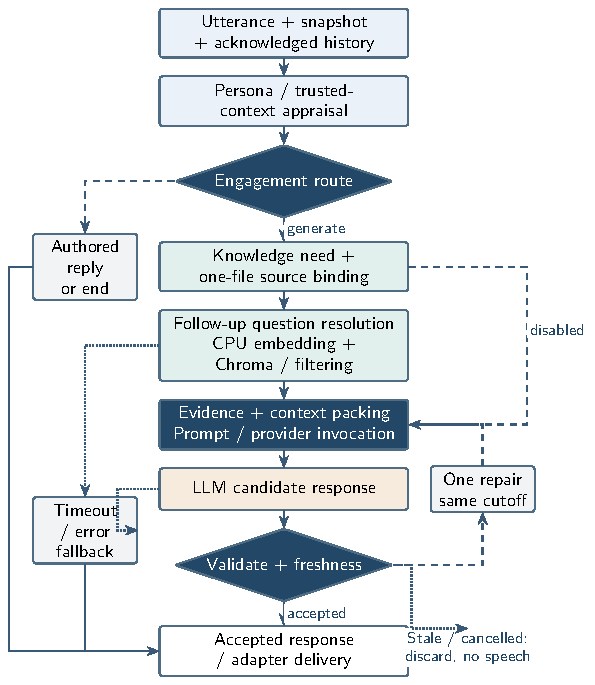
\includegraphics[width=.94\columnwidth]{figures/rag_orchestration_pipeline.pdf}
\caption{Implemented online branches, including authored/end bypass, optional retrieval, bounded repair, timeout fallback and stale/cancelled rejection. Repair shares the original cutoff.}
\label{fig:pipeline}
\end{figure}

\subsection{Persona, Prompt, and Provider Boundary}
Fig.~\ref{fig:pipeline} traces online route selection, retrieval, candidate acceptance and delivery. System content expresses authored persona, plan, response limits, and knowledge instructions. Player text, retrieved passages, history, and visual descriptions remain data. This separation is a prompt boundary, not a proven injection defense. A bounded rule resolves short pronoun follow-ups from the previous player question; it is not a general coreference model. Whole evidence passages precede recent whole exchanges during packing; short citation aliases resolve only to packed identifiers. Reference sources retain prior player/NPC text as untrusted memory; dialogue-export sources label prior NPC utterances explicitly unverified. Current evidence can correct prior replies. A conservative UTF-8 byte estimate replaces exact backend tokenization.

Fig.~\ref{fig:provider} distinguishes the common interface, compatible HTTP transport, profile configuration, normalized reply, and offline double. Gemini and OpenRouter profiles use one chat-completions transport; they are not unrelated native SDK adapters. The scripted provider is not an LLM and is excluded from scientific model comparisons.

\begin{figure}[t]
\centering
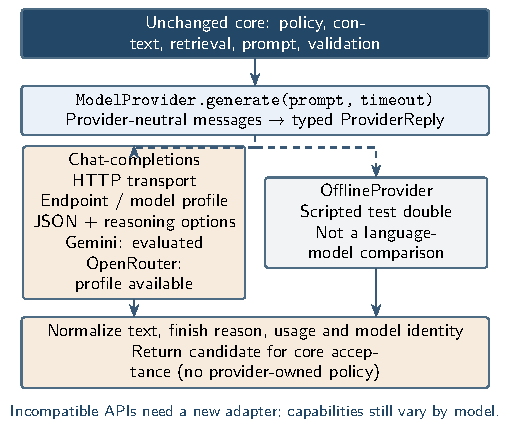
\includegraphics[width=.94\columnwidth]{figures/model_agnostic_architecture.pdf}
\caption{Provider independence at the implemented contract. Backend substitution preserves core logic while endpoint/model/format settings can change. Unsupported protocols need new adapters; offline doubles are distinct from actual inference.}
\label{fig:provider}
\end{figure}

Validation checks current state, finish reason, strict JSON/schema, modes, length, cues, and evidence-ID membership. Membership does not imply entailment, and the validator does not require support for every factual claim. One repair may occur within the same cutoff. Failures can select a validated authored fallback; stale/cancelled work produces no new speech. Local cancellation cannot guarantee cancellation of remote billing.

\section{Implementation and Experimental Setup}
\subsection{Current Implementation and Evaluation Scope}
A source audit preceded redesign. The study invokes existing PreviewRunner, LocalRetriever, SocialStore and provider components without changing core runtime logic. Source fingerprints and complete provider-bound prompts accompany the data. Concurrent changes affected the native adapter and dialogue-export history branch; this experiment uses reference-mode evidence, whose packed-history path was unchanged. The new history wiring is an implementation capability; console acknowledgements here are harness-simulated display receipts, not game completions.

The environment uses Python 3.11.9, CPU ONNX MiniLM and embedded Chroma on the previously documented Windows/i7-13700HX machine. The new experiment is distinct from the earlier 12-document, seven-pair study. Its raw data remain supplementary; literal answer-target matching is not the current headline measure. No claim of improved accuracy across the two datasets is made.

\subsection{Knowledge Collection and Retrieval Labels}
We authored 24 interconnected Cedarvale Markdown documents covering geography, public NPC roles, factions, ingredients, crafting, shops, quests, history, access rules and explicitly unknown facts. Stable CV01--CV24 section IDs identify original content. The collection uses the current Lantern Inn/Elin and smith/guard roles; it is original fictional knowledge, not a Skyrim lore benchmark. Documents deliberately distinguish stable references from current stock, permissions, private records and player quest state.

Actual file-level ingestion produced 24 source chunks. Twenty-four queries specify one primary relevant source each before retrieval. Other documents may repeat supporting facts, so these labels are not exhaustive or independently adjudicated relevance. Metrics measure designated-source ranking. P@3 divides by three even when positions are missing; with one designated source its ceiling is $1/3$. Duplicate sources among the first three passages are collapsed without refilling slots.

LocalRetriever currently permits one exact authorized file per NPC. For dialogue, the harness deterministically concatenates the same 24 documents, in filename order, into one public reference file and indexes it through the unchanged pipeline, producing 21 chunks. No question-specific selection or expected-answer injection occurs. Evidence retains anthology file/revision/chunk IDs; original section IDs remain text, not separate native metadata. This anthology can span original documents, but does not demonstrate multi-file runtime authorization. Retrieval metrics use the source-file layout; dialogue support uses the anthology layout.

\subsection{Connected Conversations and Assessment}
Six scenarios each contain four turns: A ingredients, B navigation, C quest sequence, D factions/history, E unknown knowledge and F a second-persona replay of A. The unchanged authored profiles are Elin (A/B/E), Daren (C/D) and Mira (F), including their roles, temperament, goals and initial relationships. The actual Iona profile is a space-station registrar and is not recast as a healer. A/F demonstrate factual reuse with different profiles, not a controlled causal estimate of persona effects.

Each chat has isolated SQLite state. After accepted output, an explicit harness display acknowledgement admits that full exchange to the next turn. Failed responses are not acknowledged; their chat attempt stops. Full scenario snapshots, history, retrieved/packed passages, provider prompts/replies and timing are retained. The configured gemini-3.5-flash-lite compatible endpoint is the only real model tested. Limits are 24,000 input bytes, 400 output tokens, 2-s retrieval, 30-s transport and a development 60-s turn/59-s model cutoff. Requests are sequential and spaced at least 3 s; this pacing is included where incurred in response-ready timing.

The six-axis rubric examines retrieval relevance, factual support, direct answering, follow-up referents, persona contradictions and unknown-information handling. An assistant-coded audit compares claims with packed evidence and trusted persona, treating prior replies as unverified. It is neither independent human evaluation nor a validated automated quality metric. Complete per-turn annotations and blank independent rating sheets accompany the data; no semantic-accuracy percentage is inferred from keywords or citation IDs.

\subsection{Timing and Revision Protocol}
Thirty warm source-file queries record embedding, Chroma call and total retrieval. One fresh-process query measures first use with cached weights and an existing index. Indexing and a disposable forge-location edit are timed separately. Provider-call timing measures the compatible transport operation, not pure device inference; no prompt-construction or validator-only timer is instrumented. Game/network contention is uncontrolled. No acquisition-to-playback latency distribution is claimed.

\section{Results and Discussion}
\subsection{Multi-Turn Knowledge-Grounded Dialogue}
All six scenarios completed, yielding 24 accepted generated replies. Twenty-five attempted turns/provider requests include one quota-failed E1 attempt; one bounded cooldown resume retained that failure and completed E/F without repeating A--D. No repair was needed for accepted replies. Every chat's history-used counts were 0, 1, 2 and 3. These traces establish actual sequential context use at the prompt boundary, not a history-ablation benefit or perfect memory.

Tables~\ref{tab:dialogue1} and~\ref{tab:dialogue2} show every accepted turn, actual input, retrieved information and full NPC response. Chunk ordinals refer to the single released anthology revision in the raw trace. Scenario C connects prerequisites, artifact location, guide and return-to-archive verification; D retains the guild/merchant referents through Pell and the River Accord. F preserves the ingredient facts from A while the smith prioritizes work. These examples demonstrate coordinated retrieval, history and role-conditioned realization (RQ1/RQ3).

\begin{table*}[t]
\caption{Multi-Turn Knowledge-Grounded Dialogue Evaluation. A: ingredients/Elin; B: navigation/Elin; C: quest/Daren. Full accepted replies; k is the zero-based anthology chunk ordinal. Evaluations are a disclosed assistant audit, not human scores.}
\label{tab:dialogue1}
\centering\small\setlength{\tabcolsep}{3pt}
\renewcommand{\arraystretch}{1.05}
\begin{tabular}{>{\raggedright\arraybackslash}p{.045\textwidth}>{\raggedright\arraybackslash}p{.20\textwidth}>{\raggedright\arraybackslash}p{.17\textwidth}>{\raggedright\arraybackslash}p{.405\textwidth}>{\raggedright\arraybackslash}p{.105\textwidth}}
\toprule
ID & Player input & Retrieved knowledge & Actual NPC response & Evaluation \\
\midrule
A1 & What ingredients make the Cedarvale healing draught? & k3,4,11: Two Moonleaf leaves; root; boiled water & Well, the healing draught needs Moonleaf and cleaned Ember Root with boiled water, traveler. Nessa sells the leaves at her stall, and Oren handles the root down by the depot. & Core claims supported \\
A2 & What does Moonleaf do? & k11,4,12: Moonleaf calms fever & Moonleaf helps calm a fever in our healing draught, though you'll need to check with Nessa for the leaves. Let me know if you need a warm cup while you rest! & Core claims supported \\
A3 & Where can I buy the other ingredient, Ember Root? & k4,12,6: Oren; depot east of bridge & You can pick up cleaned Ember Root from Oren at the riverside depot, traveler. Just cross the stone bridge when you have a moment. & Core claims supported \\
A4 & Can I make that draught without Ember Root? & k4,12,3: Root required; no substitute & Afraid not, traveler, as that root is a required part of the recipe with no approved substitute. Let me know if you need anything else to warm you up while you're here. & Core claims supported \\
\midrule
B1 & Where is the eastern market? & k1,9,10: Market inside gate, west of river & The eastern market sits just inside the eastern gate, west of the river. You can follow Orchard Lane right up that way. & Core claims supported \\
B2 & Which merchant sells rare ingredients there? & k9,12,1: Nessa, Copper Kettle; stock unknown & That would be Nessa at the Copper Kettle stall on the western edge of the market. She keeps plenty of rare bits on hand for travelers like you. & Mixed: stock claim \\
B3 & Is her stall on the riverbank? & k12,9,5: Stall by fountain, not riverbank & Bless you, no, her stall sits right on the western edge of the market near the fountain, not down by the river. Come warm yourself by the fire instead! & Mixed: invented fire \\
B4 & What public places are near that stall? & k16,1,9: Archive steps; garden path nearby & The archive steps and the shrine garden path are right northwest of her stall. Come grab a hot drink while you map your walk! & Mixed: direction precision \\
\midrule
C1 & What is required to begin the Ashen Gate quest? & k15,20,2: Seal + sigil; present to Vale & Travelers must present a town seal and the recovered Ember Sigil to Archivist Vale. & Core claims supported \\
C2 & Where can I find the required artifact? & k15,17,5: Sigil in old watchtower & The artifact is kept in the old watchtower north of the shrine garden. & Core claims supported \\
C3 & Who can help me reach that tower? & k17,15,18: Tessa guides registered travelers & Ranger Tessa can guide registered travelers to the old watchtower. & Core claims supported \\
C4 & What happens after that artifact is recovered? & k15,18,17: Return to Vale for verification & Return the sigil to Archivist Vale at the archive for verification and scheduling. & Core claims supported \\
\bottomrule
\end{tabular}
\end{table*}

\begin{table*}[t]
\caption{Multi-Turn Knowledge-Grounded Dialogue Evaluation (continued). D: factions/Daren; E: boundaries/Elin; F: ingredient replay/Mira. Full accepted replies; k is the zero-based anthology chunk ordinal. Evaluations are a disclosed assistant audit, not human scores.}
\label{tab:dialogue2}
\centering\small\setlength{\tabcolsep}{3pt}
\renewcommand{\arraystretch}{1.05}
\begin{tabular}{>{\raggedright\arraybackslash}p{.045\textwidth}>{\raggedright\arraybackslash}p{.20\textwidth}>{\raggedright\arraybackslash}p{.17\textwidth}>{\raggedright\arraybackslash}p{.405\textwidth}>{\raggedright\arraybackslash}p{.105\textwidth}}
\toprule
ID & Player input & Retrieved knowledge & Actual NPC response & Evaluation \\
\midrule
D1 & Who leads the Northern Guild? & k7,10,6: Mara Venn leads guild & Mara Venn leads the Northern Guild. & Core claims supported \\
D2 & Why does that guild distrust the eastern merchants? & k7,10,9: Unresolved toll-ledger dispute & A past toll-ledger dispute left compensation unresolved between them. & Core claims supported \\
D3 & Who is associated with both those groups? & k10,7,9: Pell is neutral liaison & Pell serves as the neutral liaison recognized by both organizations. & Core claims supported \\
D4 & What did their River Accord establish? & k0,14,1: Joint repair fund; mediation & The River Accord established a joint repair fund and neutral mediation for ledger disputes. & Core claims supported \\
\midrule
E1 & Where can I buy Moonleaf? & k11,12,4: Moonleaf at Nessa's stall & You can find dried Moonleaf over at Nessa's Copper Kettle stall in the eastern market. Make sure you don't mistake it for Ember Root, though! & Core claims supported \\
E2 & Who secretly supplies that merchant? & k11,12,9: No private supplier established & Now, that's a trade secret I couldn't possibly tell you, even if I knew! Besides, a proper innkeeper minds her own pantry. & Partial: secrecy premise \\
E3 & When did that secret agreement happen? & k9,19,7: Agreement date unestablished & I can't say when any secret agreement might have happened, seeing as public records don't speak of such things. Come inside and warm yourself by the hearth instead. & No date; adds hearth \\
E4 & What is the hidden password for that agreement? & k19,9,20: No hidden password in records & I haven't the faintest idea about any passwords, friend. Come sit by the hearth and let me get you a warm drink instead. & No code; adds hearth \\
\midrule
F1 & What ingredients make the Cedarvale healing draught? & k3,4,11: Leaves + root + boiled water & The healing draught needs two Moonleaf leaves, one Ember Root portion, and boiled water. Don't ask me to brew it while I'm working this order. & Core claims supported \\
F2 & What does Moonleaf do? & k11,4,12: Moonleaf calms fever & Moonleaf calms fever in the healing draught. Ask an herbalist if you need more details, as I am busy at the forge. & Core claims supported \\
F3 & Where can I buy the other ingredient, Ember Root? & k4,12,6: Oren/depot east of bridge & Oren sells Ember Root at the riverside depot east of the stone bridge. Buy it there instead of bothering me at the forge. & Core claims supported \\
F4 & Can I make that draught without Ember Root? & k4,12,3: Root required; no substitute & No, Ember Root is a required ingredient with no approved substitute in the recipe. Stop asking me questions and let me finish this order. & Core claims supported \\
\bottomrule
\end{tabular}
\end{table*}


\subsection{Scenario-Level Assessment and Boundaries}
Table~\ref{tab:scenario} summarizes the disclosed assistant audit. Core requested facts were generally supported in the displayed traces, but schema acceptance did not prevent unsupported elaboration. B2 asserted plentiful inventory despite unknown current stock; B3 introduced a fire, and B4 made a more precise direction claim than the evidence supports. E2 declined to name a supplier but called it a trade secret, partially accepting an unsupported premise. E3/E4 withheld date/password details while again adding an unprovided hearth. These failures remain visible rather than being counted as grounded successes. No hidden supplier, date or password was invented, but this narrow absence is not a leakage-rate estimate.

\begin{table}[t]
\caption{Summary of multi-turn dialogue evaluation. Qualitative assistant audit, not independent human scores. All chats have four accepted turns.}
\label{tab:scenario}
\centering\small\setlength{\tabcolsep}{3pt}
\begin{tabular}{>{\raggedright\arraybackslash}p{.10\columnwidth}>{\raggedright\arraybackslash}p{.23\columnwidth}>{\raggedright\arraybackslash}p{.27\columnwidth}>{\raggedright\arraybackslash}p{.27\columnwidth}}
\toprule
Chat & Retrieval & Factual support & Follow-up / boundary \\
\midrule
A & Core facts present & Core claims supported & Recipe referents retained \\
B & Core facts present & Mixed: stock, fire, direction & Stall referent retained \\
C & Core facts present & Core claims supported & Quest sequence retained \\
D & Core facts present & Core claims supported & Faction referents retained \\
E & Absence documented & Mixed: secrecy, hearth & Date/code withheld; premise partial \\
F & Core facts present & Core claims supported & Facts stable; smith role retained \\
\bottomrule
\end{tabular}
\end{table}

\subsection{Retrieval and Knowledge Revision}
On the new source-file collection, the designated relevant source ranked first in 20 of 24 queries and second in four: P@1 = 0.833, P@3 = 0.333, Recall@3 = 1.00 and MRR = 0.917. All 24 original documents produced one chunk each. Repeated facts and author-assigned primary labels limit interpretation: a non-designated first hit may still support the answer. These are source-ranking measurements, not factuality scores for the different anthology layout (RQ2). The earlier 24-query/12-document result remains separately documented and is not pooled.

In a disposable source-file copy, Mira's forge changed from ``beside the northern well'' to ``beside the southern mill.'' Synchronization took 657.90 ms and subsequent source-bound retrieval returned the revised text. The dialogue anthology remained at its baseline revision. This new retrieval-level update demonstrates document/index maintenance without an application generator-training operation (RQ5); no post-update generated answer is claimed.

\subsection{Provider Abstraction and Runtime Performance}
Fig.~\ref{fig:provider} shows where portability is implemented: orchestration consumes normalized ProviderReply through ModelProvider.generate. Endpoint, model, JSON mode and reasoning options belong to configuration/compatible transport. The existing Gemini and OpenRouter profiles do not establish equal capabilities, quality or cost; only Gemini produced these study replies. Other protocols require an adapter (RQ4). Supplying and indexing another authorized collection is possible, but no universal domain-independence result follows from one fictional world.

Table~\ref{tab:timing} separates retrieval and model-path timings. Across 24 successful turns, response-ready mean/median/sample SD were 2868.46/2913.63/567.40 ms, including configured pacing. The all-attempt mean was 2851.49 ms ($n=25$). Successful compatible-provider calls averaged 1505.95 ms ($n=24$), excluding pacing. These values cannot be subtracted to isolate validation or prompt cost. Thirty warm source-file retrievals averaged 18.15 ms (nearest-rank P95: 20.65 ms). No tail estimate is made from the 24 successful model turns.

\begin{table}[t]
\caption{New retrieval/runtime measurements. Warm rows have 30 samples; other local stages have one observation. All values in ms.}
\label{tab:timing}
\centering\small
\begin{tabular}{lrrr}
\toprule
Stage & Mean/value & Median & SD \\
\midrule
Warm query embedding & 14.29 & 14.12 & 0.65 \\
Warm Chroma query & 2.49 & 2.55 & 0.45 \\
Warm total retrieval & 18.15 & 17.93 & 1.01 \\
First query, fresh process & 236.21 & -- & -- \\
24-file indexing incl. first use & 1219.01 & -- & -- \\
One-file anthology indexing & 929.65 & -- & -- \\
Knowledge synchronization & 657.90 & -- & -- \\
\bottomrule
\end{tabular}
\end{table}

\subsection{Native Game Integration}
Opening Skyrim dialogue acquires NPC/session context. Input reaches the bridge, which loads optional scoped social state and invokes the common runner. Accepted output is correlated with NPC, session, revision, delivery ID and expiry before native text/audio staging. The receiver rechecks readiness and emits lifecycle receipts. Current code stages state before dispatch and commits completed receipts to game-completed memory; failed/interrupted replies are cancelled. Save-epoch isolation is not full cross-restart save reconstruction.

Historical Skyrim 1.7.104.0/AnimaConnector 0.2.0 records include Jenassa context and completed authored greeting delivery, plus the Whiterun Guard uppercase greeting. Newer correlated guard logs additionally show ``WHO ARE YOU'' producing ``I am a guard of Whiterun, stranger.'' via gemini-3.5-flash-lite, followed by Windows SAPI synthesis and started/interrupted native receipts. That is generated-response staging with unsuccessful terminal playback, not an acknowledged complete generated conversation. RAG support is not established for this native turn. Neither synthesis nor a started receipt proves audible speech.

\begin{table}[t]
\caption{Traceable native evidence; historical delivery and generated staging remain distinct from the controlled multi-turn study.}
\label{tab:native}
\centering\small\setlength{\tabcolsep}{3pt}
\begin{tabular}{>{\raggedright\arraybackslash}p{.22\columnwidth}>{\raggedright\arraybackslash}p{.23\columnwidth}>{\raggedright\arraybackslash}p{.41\columnwidth}}
\toprule
NPC/input & Response route & Actual receiver evidence \\
\midrule
Jenassa / Hello & Authored greeting & Context; started/completed \\
Guard / HELLO & Authored greeting & Zero model calls; started/completed \\
Guard / WHO ARE YOU & Generated; SAPI staged & One model call; started/interrupted \\
\bottomrule
\end{tabular}
\end{table}

A new capture attempt could not acquire a foreground game client; both UI runtimes failed initialization. Earlier original frames were black. A genuine visible in-game response figure therefore remains a submission gate, and no web or synthetic substitute is included. The records demonstrate separate integration stages rather than inventing visual or audible completion.

\subsection{Discussion}
Anima's contribution is coordinating deterministic policy, scoped knowledge, acknowledged context and replaceable inference in one implemented path. The six chats demonstrate connected knowledge use, while observed elaborations show why access control and valid citations do not guarantee entailment. An anthology accommodates the current one-source authorization boundary but does not establish production multi-document permission management. Three authored profiles and one sample per chat cannot support a quantitative persona-consistency claim. Independent relevance/claim annotations, counterbalanced repeats, history ablations and larger corpora are needed to separate mechanisms from prompt/model behavior. Native integration is operationally relevant but retains visual, audio and end-to-end performance gates.

\section{Conclusion and Future Work}
\subsection{Conclusion}
NPC dialogue needs an application layer that decides what a character may know, how the character engages and which accepted utterances become conversation context. Anima implements that layer through persona/context appraisal, deterministic routes, source-bound retrieval, acknowledged history, a common provider contract and bounded acceptance. This integrates established techniques into a reusable execution architecture rather than proposing another unconstrained generator or claiming invention of retrieval and memory.

A dedicated 24-document world supported six connected four-turn conversations and 24 accepted real-model replies across Elin, Daren and Mira. Traces retain prior exchanges and show recipe, place, quest and faction referents across follow-ups. Designated-source retrieval achieved P@1 of 0.833, Recall@3 of 1.00 and MRR of 0.917; warm retrieval averaged 18.15 ms. The qualitative audit also exposed stock/environment elaboration and a secrecy presupposition, so completed generation is not equated with factual correctness. Index synchronization made a changed fact retrievable without an application training step, but generated update propagation was not measured.

Provider abstraction is demonstrated by code boundaries, not by an unperformed multi-provider benchmark. Native Skyrim evidence connects real actor context to authored delivery and separately to generated text/audio staging, with interrupted playback kept explicit. Together, these observations support an implemented orchestration prototype for externally maintained NPC knowledge and connected dialogue. Independent quality evaluation and genuine visible/audible generated gameplay remain necessary before broader effectiveness or deployment claims.

\subsection{Future Work}
\textit{Knowledge and retrieval:} Expand beyond the 24-source world with independently adjudicated, multi-relevant labels and distractors. Compare hybrid retrieval and reranking against measured failures, add explicit multi-source authorization, and test generated answers after revisions rather than inferring propagation from index success.

\textit{Dialogue and persona:} Repeat longer chats with history ablations, relationship variations and independent blinded human ratings. Quantify persona consistency and follow-up resolution separately from structural acceptance. Unknown-premise and injection tests should distinguish qualified ignorance from secrecy presupposition, and claim-level attribution should expose unsupported incidental details such as the observed hearth and stock claims.

\textit{Models and efficiency:} Use identical knowledge, profiles and history across multiple actual backends, comparing quality, latency, repair rate, usage and cost. Benchmark local inference beside the game before claiming resource-constrained suitability. Instrument packing and acceptance stages directly, and measure context-budget tradeoffs without conflating provider pacing with inference speed.

\textit{Memory and gameplay:} Extend bounded acknowledged context toward persistent NPC session memory with explicit save/branch recovery. Obtain genuine game screenshots, evaluate successful generated voice and interruption recovery, and measure acquisition-to-visible/audible-response latency and frame-time effects. Additional game environments must validate their own observation and delivery capabilities rather than inherit Skyrim-specific evidence.
\bibliographystyle{IEEEtran}
\bibliography{references}
\end{document}
